\message{ !name(teoria.tex)}\documentclass[a4paper,12pt, oneside]{book}

% \usepackage{fullpage}
\usepackage[italian]{babel}
\usepackage[utf8]{inputenc}
\usepackage{amssymb}
\usepackage{amsthm}
\usepackage{graphics}
\usepackage{amsfonts}
\usepackage{listings}
\usepackage{amsmath}
\usepackage{amstext}
\usepackage{engrec}
\usepackage{rotating}
\usepackage{verbatim}
\usepackage[safe,extra]{tipa}
%\usepackage{showkeys}
\usepackage{multirow}
\usepackage{hyperref}
\usepackage{microtype}
\usepackage{fontspec}
\usepackage{enumerate}
\usepackage{physics}
\usepackage{braket}
\usepackage{marginnote}
\usepackage{pgfplots}
\usepackage{cancel}
\usepackage{polynom}
\usepackage{booktabs}
\usepackage{enumitem}
\usepackage{framed}
\usepackage{pdfpages}
\usepackage{pgfplots}
\usepackage{algorithm}
% \usepackage{algpseudocode}
\usepackage[cache=false]{minted}
\usepackage{mathtools}
\usepackage[noend]{algpseudocode}

\usepackage{tikz}\usetikzlibrary{er}\tikzset{multi  attribute /.style={attribute
    ,double  distance =1.5pt}}\tikzset{derived  attribute /.style={attribute
    ,dashed}}\tikzset{total /.style={double  distance =1.5pt}}\tikzset{every
  entity /.style={draw=orange , fill=orange!20}}\tikzset{every  attribute
  /.style={draw=MediumPurple1, fill=MediumPurple1!20}}\tikzset{every
  relationship /.style={draw=Chartreuse2,
    fill=Chartreuse2!20}}\newcommand{\key}[1]{\underline{#1}}
  \usetikzlibrary{arrows.meta}
  \usetikzlibrary{decorations.markings}
  \usetikzlibrary{arrows,shapes,backgrounds,petri}
\tikzset{
  place/.style={
        circle,
        thick,
        draw=black,
        minimum size=6mm,
    },
  transition/.style={
    rectangle,
    thick,
    fill=black,
    minimum width=8mm,
    inner ysep=2pt
  },
  transitionv/.style={
    rectangle,
    thick,
    fill=black,
    minimum height=8mm,
    inner xsep=2pt
    }
  } 
\usetikzlibrary{automata,positioning,chains,fit,shapes}
\usepackage{fancyhdr}
\pagestyle{fancy}
\fancyhead[LE,RO]{\slshape \rightmark}
\fancyhead[LO,RE]{\slshape \leftmark}
\fancyfoot[C]{\thepage}
\usepackage[usenames,dvipsnames]{pstricks}
\usepackage{epsfig}
\usepackage{pst-grad} % For gradients
\usepackage{pst-plot} % For axes
\usepackage[space]{grffile} % For spaces in paths
\usepackage{etoolbox} % For spaces in paths
\makeatletter % For spaces in paths
\patchcmd\Gread@eps{\@inputcheck#1 }{\@inputcheck"#1"\relax}{}{}
\makeatother

\title{Teoria dell'Informazione e Crittografia}
\author{UniShare\\\\Davide Cozzi\\\href{https://t.me/dlcgold}{@dlcgold}}
\date{}

\pgfplotsset{compat=1.13}
\begin{document}

\message{ !name(teoria.tex) !offset(-3) }

\maketitle

\definecolor{shadecolor}{gray}{0.80}
\setlist{leftmargin = 2cm}
\newtheorem{teorema}{Teorema}
\newtheorem{definizione}{Definizione}
\newtheorem{esempio}{Esempio}
\newtheorem{corollario}{Corollario}
\newtheorem{lemma}{Lemma}
\newtheorem{osservazione}{Osservazione}
\newtheorem{nota}{Nota}
\newtheorem{esercizio}{Esercizio}
\algdef{SE}[DOWHILE]{Do}{doWhile}{\algorithmicdo}[1]{\algorithmicwhile\ #1}
\tableofcontents
\renewcommand{\chaptermark}[1]{%
  \markboth{\chaptername
    \ \thechapter.\ #1}{}}
\renewcommand{\sectionmark}[1]{\markright{\thesection.\ #1}}
\newcommand{\floor}[1]{\lfloor #1 \rfloor}
\newcommand{\MYhref}[3][blue]{\href{#2}{\color{#1}{#3}}}%
\chapter{Introduzione}
\textbf{Questi appunti sono presi a lezione. Per quanto sia stata fatta
  una revisione è altamente probabile (praticamente certo) che possano
  contenere errori, sia di stampa che di vero e proprio contenuto. Per
  eventuali proposte di correzione effettuare una pull request. Link: }
\url{https://github.com/dlcgold/Appunti}.\\
\chapter{Introduzione agli argomenti del corso}
Si ha una sorgente che emette messaggi e li vuole mandare tramite un canale di
comunicazione, che contiene del rumore che agisce sui messaggi e li rovina. Il
destinatario per capire che il messaggio è rovinato ha varie tecniche. Una
prima cosa che potrebbe fare è chiedere di rimandare il messaggio ma sarebbe
meglio correggere \textit{in loco} e si hanno algoritmi per farlo (tra cui lo
\textbf{schema di Hamming} usando il modello del \textbf{rumore bianco}).\\
Un'altra tematica è la codifica stessa del sorgente, comprimendo flussi di dati,
senza perdere informazioni.\\
Si parlerà anche dei canali di comunicazione, delle capacità e dei
\textbf{teoremi di Shannon}. \\
Si vedranno poi le basi della crittografia, i crittosistemi storici, vari
standard etc$\ldots$
\chapter{Teoria dell'informazione}
Si hanno due sottoparti principali:
\begin{itemize}
  \item \textbf{teoria dei codici}, per individuare e correggere gli errori. Si
  studia il canale di trasmissione cercando di contrastare il rumore che c'è nel
  canale
  \item \textbf{teoria dell'informazione}, in cui il focus è la sorgente delle
  informazioni
\end{itemize}
Vediamo il classico schemino della teoria dell'informazione:
\begin{figure}[H]
  \centering
  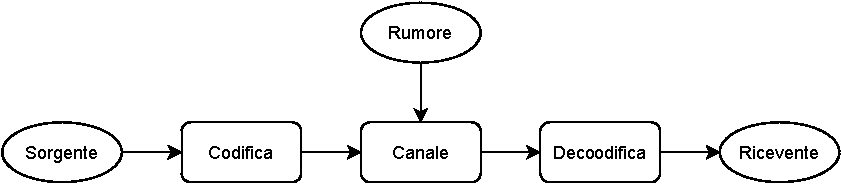
\includegraphics[width = \textwidth]{img/teo.pdf}
  \caption{Schema di un sistema generale di comunicazione tipico della teoria
    dell'informazione} 
  \label{fig:teo}
\end{figure}
Avendo:
\begin{itemize}
  \item la \textbf{sorgente} che produce segnali, dei simboli, che potrebbero
  essere continui (come la corrente), anche se noi li assumeremo come simboli di
  un alfabeto finito, avendo quindi una \textbf{sorgente discreta}
  \item i simboli, per poter essere spediti all'interno di un canale, vanno
  codificati, avendo una parte di \textbf{codifica}
  \item una volta codificati i simboli vanno nel \textbf{canale di
    trasmissione}, dove si ha del \textbf{rumore}. Tale \textit{rumore} prende
  un simbolo di quelli inseriti e lo cambia
  \item dal canale esce o il simbolo che è entrato o il simbolo modificato dal
  rumore e, tipicamente, non è immediatamente utilizzabile ma deve passare per
  una fase di \textbf{decodifica}
  \item il simbolo decodificato arriva al \textbf{destinatario}
\end{itemize}
Si hanno
alcune assunzioni sulla sorgente:
\begin{itemize}
  \item è \textbf{discreta}, i simboli emessi appartengono ad un alfabeto
  finito. Normalmente tali simboli sono $S=\{s_1, s_2,\ldots,s_q\}$
  \item i simboli vengono emessi uno alla volta ad ogni \textbf{colpo di
    clock}. Non si ha mai che in un colpo di clock non escano simboli o che ne
  escano più di uno solo 
  \item la sorgente è \textbf{senza memoria (\textit{memoryless})}, avendo che
  i simboli già usciti non influenzano per nulla il simbolo che sta per
  uscire. Ogni simbolo che esce non tiene conto del passato, \textit{è come se
    fosse il primo}
  \item è \textbf{probabilistica e randomizzata}. Si ha quindi che i simboli
  $S=\{s_1, s_2,\ldots,s_q\}$ escono con le probabilità
  $(p_1,p_2,\ldots,p_q)$. Deve valere che, ovviamente, che $p_i\in
  [0,1],\forall
  i=1,\ldots,q$. Si ha inoltre che le varie probabilità, nel loro insieme,
  devono formare una distribuzione di probabilità, avendo che:
  \[\sum_{i=1}^q p_i=1\]
  Potrei avere simboli con probabilità nulla di comparire ma nella pratica non
  è qualcosa di sensato. La sorgente la costruisco o da zero (e a quel punto
  un simbolo con probabilità nulla non lo metterei) o ho una sorgente che devo
  studiare (e qui potrei avere simboli con probabilità bassissime se non
  nulle, in tal caso bisognerebbe rivalutare l'assunzione dei simboli di
  quella sorgente). Possiamo quindi meglio dire che $p_i\in (0,1],\forall
  i=1,\ldots,q$.\\
  D'altro canto vedo se posso avere probabilità pari a 1 per un simbolo ma in
  tal caso avrei solo quello e non sarebbe interessante. Si ha quindi che:
  \[p_i\in (0,1),\forall i=1,\ldots,q\]
  \[\sum_{i=1}^q p_i=1\]
  \textit{Le sorgenti che emettono i simboli secondo  
    uno schema prefissato, deterministico, sono poco interessanti, avendo un
    comportamento banale}
\end{itemize}
Il concetto di \textit{spedire in un canale} può anche essere generalizzato in
altre ``idee'', come il disco su cui salvo dei dati e il tempo per cui li
salvo.\\ 
La parte di \textit{codifica e decodifica} può essere approfondita. Nello schema
in figura \ref{fig:teo} ci si è infatti concentrati sul canale, avendo che la
codifica serve a fare in modo che il simbolo trasmesso vada bene per essere
trasmesso nel canale. La \textbf{codifica} è a sua volta suddivisa in due parti:
\begin{enumerate}
  \item \textbf{codifica di sorgente}, che ha come obiettivo rappresentare nel
  modo più efficiente e compatto i simboli emessi dalla \textit{sorgente}. Si
  vuole quindi comprimere la sequenza di simboli (messaggi) emessi dalla
  sorgente, per impegnare meno banda possibile quando andremo a spedire. Si deve
  considerare che ogni bit in un file 
  compresso è essenziale per permettere di poter recuperare il contenuto
  compresso 
  \item \textbf{codifica di canale}, che ha quasi uno scopo opposto rispetto
  alla \textit{codifica di sorgente}, infatti ha come obiettivo quello di
  contrastare il rumore e per farlo aggiunge ridondanza al messaggio (da qui il
  discorso sull'obiettivo opposto)
\end{enumerate}
Si cerca quindi di comprimere il più possibile nella prima fase, quella di
\textit{codifica di sorgente} e di ridondare il meno possibile nella seconda,
quella di \textit{codifica di segnale}.\\
Per capire meglio quanto detto diamo alcune formalità.
\begin{definizione}
  Una \textbf{codifica} è una funzione $cod$ che prende i simboli della sorgente
  $S=\{s_1, s_2,\ldots,s_q\}$ e ad ogni simbolo $s_i$ gli assegna una stringa
  formata coi caratteri di un certo alfabeto $\Gamma$, l'\textbf{alfabeto
    della codifica}. Le stringhe di $\Gamma^*$ sono tutte quelle costruite
  sull'alfabeto $\Gamma$ di lunghezza arbitraria e finita, compresa la stringa
  vuota $\varepsilon$, che posso quindi formare coi simboli di $\Gamma$. Quindi
  ad ogni $s_i\in S$ assegno un $\gamma_i\in Gamma^*$, avendo che:
  \[cod:S\to \Gamma^*\]
  generalmente si ha che:
  \[|\Gamma|<|\Sigma|\]
  e quindi i simboli di $\Sigma$ sono mappati da $cod$ in  sequenze  di  simboli
  di $\Gamma$, a meno che non si ritenga accettabile il fatto che due o più
  simboli di $\Sigma$ vengano mappati nellostesso simbolo di $\Gamma$. \\
  \textit{Più avanti nel corso vedremo casi in cui $|\Gamma|>|\Sigma|$}
\end{definizione}
Si hanno quindi i simboli $S=\{s_1, s_2,\ldots,s_q\}$ che escono con
probabilità $(p_1,p_2,\ldots,p_q)$ e che vengono codificati con le stringhe
$\gamma_1,\gamma_2,\ldots,\gamma_q$. Le varie $gamma_i$ sono dette
\textbf{codeword}. Chiamando $l_i=|\gamma_i|$ la lunghezza 
di tali stringhe si ha che tali stringhe hanno associati i vari
$l_1,l_2,\ldots,l_q$.\\
L'obiettivo quindi della \textit{codifica di sorgente} è quello di minimizzare
la lunghezza media $L$ delle stringhe, avendo quindi una media pesata (pesata
sulle probabilità):
\[L=\sum_{i=1}^q p_i\cdot l_i\]
Tenendo conto delle probabilità, per minimizzare $L$, si deve, avendo a che fare
con termini che sono tutti $>0$ (avendo supposto che non si hanno probabilità
nulla e avendo che una codeword pari alla stringa vuota ha poco senso), fare in
modo che i termini siano tutti il più piccolo possibile. Dato che le probabilità
sono date mentre la codifica la sto costruendo, calcolando le codeword e di
conseguenza le loro lunghezze, devo fare in modo che se la probabilità è grande
la lunghezza deve essere piccola. Se invece la probabilità è piccola posso
permettermi una lunghezza più grande. Parto quindi dai simboli con probabilità
più grande e inizio a usare codeword più piccole possibili, usando via via
quelle più lunghe. \\
Un'idea simile è usata nel \textit{codice Morse} dove le
lettere meno comuni hanno le sequenze più lunghe di punti, linee e spazi (avendo
una codifica ternaria). La lettera più comune, la ``e'', ha infatti solo con un
punto, la codifica più breve mentre le meno comuni hanno sequenze multiple di
punti, linee e spazi che le separano (e gli spazi contano nella lunghezza di
queste codeword).\\
Noi non sappiamo in anticipo che messaggi verranno prodotti dalla sorgente e
quindi le codeword vanno studiate passo a passo, valutando i simboli più
probabili per associare le codeword più brevi e i meno probabili per le
codeword più lunghe.\\
Analizziamo meglio i codici, le codeword. Possono essere:
\begin{enumerate}
  \item \textit{a lunghezza fissa}, ovvero si ha che $l_1=l_2=\cdots=L_q$
  \item \textit{a lunghezza variabile}, avendo che ogni codeword può avere
  lunghezza diversa
\end{enumerate}
Ne segue quindi che il discorso di minimizzare $L$ ha senso solo in presenza di
\textit{codeword a lunghezza variabile} (potendo decidere per ogni simbolo che
codeword associare), avendo la \textbf{codifica a lunghezza variabile}.\\
Con \textit{codeword a lunghezza fissa} avrei tutte le $l_i$ uguali e quindi
avrei, avendo $l_i=l,\forall i$:
\[L=\sum_{i=1}^q p_i\cdot l_i \sum_{i=1}^q p_i\cdot l =l\cdot\sum_{i=1}^q
  p_i=l\cdot 1 = l\]
avendo, come facilmente intuibile, che la lunghezza media è la lunghezza fissa
stessa. Si hanno codifiche a lunghezza fissa, come banalmente numeri a 64bit
etc$\ldots$ in tal caso si parla di \textbf{codici a blocchi}.\\
Usando codifiche a lunghezza fissa si hanno anche esempi interessanti come
quello del \textit{codice pesato}, detto \textbf{codice pesato 01247}. Il nome
deriva dal fatto che si possono codificare le cifre da 0 a 9 (da 1 a 9 con poi
lo 0 dopo il 9) sotto forma di stringhe di 5 bit usando i pesi 0,1,2,4,7
associati a ciascun bit. Vediamo la tabella con la codifica di questo codice:
\begin{table}[H]
  \centering
  \begin{tabular}{c|ccccc} 
    & 0 & 1 & 2 & 4 & 7 \\
    \hline
    1 & 1 & 1 & 0 & 0 & 0 \\
    2 & 1 & 0 & 1 & 0 & 0 \\
    3 & 0 & 1 & 1 & 0 & 0 \\
    4 & 1 & 0 & 0 & 1 & 0 \\
    5 & 0 & 1 & 0 & 1 & 0 \\
    6 & 0 & 0 & 1 & 1 & 0 \\
    7 & 1 & 0 & 0 & 0 & 1 \\
    8 & 0 & 1 & 0 & 0 & 1 \\
    9 & 0 & 0 & 1 & 0 & 1 \\
    0 & 0 & 0 & 0 & 1 & 1
  \end{tabular}
\end{table}
Si nota che ogni codeword ha sempre 3 bit pari a 0 e due bit pari a 1, avendo un
\textbf{codice 2-su-5}. Banalmente i pesi si associano ai numeri 0,1,2,4,7 in
modo tale che essi, sommati, formino il numero voluto (ad esempio per 1 avrò i
pesi su 0 e 1, per 9 su 2 e 7 etc$\ldots$). L'unico caso è il caso dello 0, che
non può essere ottenuto come somma di due pesi (spesso si hanno nei codici casi
speciali da gestire a parte). Per lo 0 viene quindi presa una codeword non usata
per altri numeri e quindi l'unica scelta possibile è avere i pesi su 4 e 7
(visto che farebbe 11).\\
Su un totale ci 5 bit, avendo due bit a 1 e tre bit a 0, posso avere un numero
di codeword pari a:
\[n={{5}\choose{2}}=10\]
avendo che i 5 bit sono associati ai 5 elementi dove 1 segnala che ``sto usando
quel peso'', prendendo quindi i sottoinsiemi di due elementi a partire da un
insieme di cinque elementi, ovvero ``in quanti modi posso formare sottoinsiemi
che contengono due elementi a partire da un insieme di cinque elementi'' o detto
altrimenti ``quanti sono i modi in cui posso disporre due uni all'interno di una
stringa di cardinalità cinque''.\\
In un linguaggio di programmazione privo di una struttura dati dedicata posso
simulare un insieme di questo tipo tramite un vettore di bit (con 1 se
l'elemento associato all'indice c'è).\\
\textit{Il codice a barre è detto \textbf{codice 39} ed è un \textbf{codice
    3-su-9}}. \\
In merito alla \textbf{decodifica} si ha che anch'essa sarà di due tipi:
\begin{enumerate}
  \item \textbf{decodifica di canale}, vedendo e c'è stato un errore di
  trasmissione ed eventualmente correggendolo in automatico se il codice mi
  consente di farlo
  \item \textbf{ulteriore decodifica} che non è esattamente una \textit{codifica
    di sorgente} ma quanto una \textit{trasformazione}, dove le
  \textit{codeword} vengono trasformate nel formato leggibile dal
  \textbf{ricevente} 
\end{enumerate}
\section{Codici per individuare errori}
Ci concentriamo ora sulla \textit{codifica di canale} ignorando per ora la
\textit{codifica di sorgente}, avendo come obiettivo l'aggiunta di ridondanza a
simboli, che si suppongono già codificati con codeword, in modo tale che in
queste codeword, spedite nel canale dove eventualmente si possono avere
modifiche causate dal rumore, vengano eventualmente riconosciuti (ed
eventualmente corretti) errori in fase di \textit{decodifica}.\\
\textit{Parlando di codici per individuare errori solitamente, nei disorsi, si
  ha che $|\Gamma|<|\Sigma|$}
Qualora il ricevente con la sua decodifica si accorga che è successo qualcosa ma
non si è in grado di 
correggere quel qualcosa si hanno i cosiddetti \textbf{codici per individuare
  gli errori (\textit{error detection codes})}. Nel caso in cui il ricevente con
la sua decodifica si accorga dell'errore ci si chiede anche se può correggerlo
autonomamente senza chiedere che la sorgente spedisca nuovamente il
messaggio. Non sempre questa cosa si può fare ma quanto accade si parla di
\textbf{codici a correzione d'errore (\textit{error correction codes})}.\\
Vediamo come capire se un messaggio ricevuto è valido.\\
Si supponga di spedire un pacchetto di $n$ bit (ma potrebbe essere qualsiasi
altra cosa ma per praticità prendiamo un bit) nel canale e che da esso esca un
certo pacchetto sempre di $n$ bit (per il rumore potrebbe non essere lo stesso).
\begin{definizione}
  Definiamo il \textbf{controllo di parità}. \\
  Avendo una sequenza di $n$ bits in
  cui si ha $n-1$ bits, dette \textbf{cifre di messaggio} di
  \textbf{messaggio vero}, che chiameremo
  \textbf{\textit{msg}} e un bit che è la \textbf{cifra di controllo}, che
  chiameremo \textbf{\textit{check}}. Le cifre di messaggio si indicano con
  $\circ$ mentre la cifra di controllo con $\times$ e quindi il messaggio è del
  tipo:
  \begin{table}[H]
    \centering
    \begin{tabular}{|c|c|c|c|c|c|c|}
      \hline
      $\circ$&$\circ$&$\circ$&$\circ$&$\cdots$&$\circ$&$\times$\\
      \hline
    \end{tabular}
  \end{table}
  avendo $n-1$ $\circ$ e un solo $\times$ (che potrebbe anche non essere in
  fondo, basta avere coscienza della posizione nel pacchetto, concordando la
  cosa tra mittente e ricevente).\\
  Si ha che:
  \begin{itemize}
    \item chi spedisce ha le cifre di messaggio e deve calcolare la cifra di
    controllo
    \item chi riceve controlla che la cifra di controllo sia coerente con le
    cifre di messaggio
  \end{itemize}
  Nell'\textbf{error detection code} il ricevente è solo in grado di capire che
  la sequenza non è valida ma per farlo bisogna assumere di avere limitazioni
  nella sequenza di $n$ bit che è entrata nel canale. Questa limitazione è che
  gli $n$ bit entranti nel canale siano una \textbf{codeword valida}, avendo
  che, preso un sottoinsieme $M$ di tutto l'insieme di $n$ bit, ovvero
  $M\subseteq\{0,1\}^n$, $M$ è un insieme di \textit{codeword valide}. Quindi
  solo un messaggio appartenente a $M$ può entrare nel canale. Fatta questa
  premessa, quando esce un messaggio, ho che, a causa del rumore, questo
  messaggio viene rovinato, non avendo più un messaggio
  valido (cosa che viene capita dal ricevente). \textit{Purtroppo può succedere
    che il rumore trasformi un messaggio valido in un altro messaggio valido ma
    non considereremo questa opzione per ora}. \\
  Nel \textbf{controllo di parità semplice} il pacchetto di $n$ bit, come visto
  è formato da $n-1$ bit di messaggio e un bit di controllo, la \textbf{check
    digit}. Si procede quindi, ricordando che siamo in un caso binario, a
  contare il numero di $1$ nei primi $n-1$ bit e se questo è dispari setto il
  bit di check a $1$ e si nota che così il numero di $1$ nel pacchetto intero
  di $n$ bit diventa pari, avendo la cosiddetta \textbf{parità pari} (ovvero
  ogni sequenza valida ha un numero pari di $1$). Controllando il numero di $1$
  il ricevente capisce se il rumore ha modificato il messaggio anche se non può
  capire cosa è successo (avendo quindi che il \emph{controllo di parità
    semplice} è solo un \emph{error detecting code} e non un \emph{error
    correcting code}). Non potendo fare nulla, in caso di errore identificato,
  il ricevente può solo chiedere al mittente di inviare nuovamente il messaggio.
  Qualora il rumore modificasse il messaggio in modo tale che si abbia comunque
  un numero apri di $1$ si rientrerebbe nella casistica sopra descritta in cui
  il rumore forma ancora un messaggio valido. Questa cosa può succedere se, nel
  caso binario, il rumore modifica un numero pari di cifre e quindi il
  \emph{controllo di parità semplice} funziona solo se viene modificato un
  \emph{numero dispari di cifre}.
  
\end{definizione}
Vediamo quindi meglio come calcolare la \textbf{check digit}.\\
Si rinominiamo gli $n$ bit come:
\[x_1x_2\cdots x_{n-1}\,y\]
quindi con $y$ \textit{check digit}.\\
Si ha che, con $\oplus$ \textit{xor}:
\[y=x_1\oplus x_2\oplus\cdots\oplus x_{n-1}\]
Ricordando che:
\begin{table}[H]
  \centering
  \begin{tabular}{c|c|c|c}
    $a$& $b$ & $a\land b$& $a\oplus b$\\
    \hline
    0 & 0 & 0 &0\\
    0 & 1 & 0 & 1\\
    1 & 0 & 0 &1\\
    1 & 1 & 1 & 0\\    
  \end{tabular}
\end{table}
quindi vale $1$ sse i due bit in input sono diversi ma questo non ci aiuta su
$n-1$ input. Altrimenti si ha che vale $1$ sse il numero di $1$ in input è
dispari e questo ci aiuta su $n-1$ input infatti la generalizzazione dello
\textit{xor} a più di due input è detta \textbf{funzione di parità}. Un altro
punto di vista per considerare lo \textit{xor} è quello della \textbf{somma a
  modulo 2} usando la notazione:
\[y=\bigoplus_{i=1}^{n-1}x_i=\sum_{i=1}^{n-1}x_i\mbox{ mod } 2\]
avendo che faccio prima la somma e poi il modulo 2 mi dice 0 se è pari e 1 se è
dispari. \\
Si ha inoltre una relazione interessante tra le formule scritte usando solo
$\oplus$ e $\land$ nella cosiddetta \textbf{forma algebrica normale
  (\textit{ANF})}. Queste formule booleane possono essere trasformate in formule
aritmetiche con \textit{modulo 2}, quindi in $\mathbb{Z}_2$ dicendo che lo
\textit{xor} equivale alla \textit{formula modulo due} e l'\textit{and} al
\textit{prodotto modulo due} (la cosa vale in entrambi i versi).\\
La funzione di parità è così usata che in tutti i microprocessori, fin dagli
anni settanta, si ha un \textit{flag di parità} tra i flag della CPU, che viene
settato come appena visto a seconda dei bit caricati su un registro particolare
(a volte detto \textit{accumulatore}). Tale calcolo è facilmente mappabile in
un circuito, avendo che lo \textit{xor} gode della proprietà associativa (avendo
un circuito che fa un albero di porte \textit{xor}).
\newpage
Posso anche simulare lo \textit{xor} con un \textbf{automa a stati finiti}, con
due stati ``pari'' e ``dispari'', con il ``pari'' stato iniziale (diciamo che
input vuoto è pari):
\begin{center}
  \begin{tikzpicture}[shorten >=1pt,node distance=3cm,on grid,auto]
    \node[state, initial, accepting] (q_0) {$pari$};
    \node[state, accepting] (q_1) [right=of q_0] {$dispari$};
    \path[->]
    (q_0) edge [bend left = 25] node {1} (q_1)
    edge [loop above] node {0} ()
    (q_1) edge [bend left = 25] node {1} (q_0)
    edge [loop right] node {0} ();
  \end{tikzpicture}
\end{center}
Questo metodo ha senso se il canale è pochissimo rumoroso, avendo pochissima
probabilità di avere la modifica di un bit e ancora meno di due (due modifiche
si ricorda che non verrebbero rilevate essendo pari), così poca da poter
ipotizzare che non avvengano mai due errori (e se mai dovesse succedere
bisognerà valutare l'impatto del problema e le conseguenze). Stiamo assumendo
quindi che la \textbf{probabilità d'errore} può essere \textbf{trascurabile}
infatti canali di buona qualità dovrebbero sbagliare non più di un bit su un
milione, per canali più affidabili anche uno su un miliardo. Possiamo quindi
trascurare che possano accadere due errori e dire che il \textbf{controllo di
  parità} va bene. \\
Parliamo ora meglio di \textbf{ridondanza}, definendola formalmente.
\begin{definizione}
  La \textbf{ridondanza} $R$ è definita come:
  \[R=\frac{\mbox{il numero totale di simboli/cifre spediti}}{\mbox{numero di
        simboli/cifre che sono effettivamente parte del messaggio}}\] 
  Nel caso del \emph{controllo di parità} i simboli che vogliamo spedire sono
  $n$ bit a fronte di $n-1$ bit di vero messaggio. Si ha quindi:
  \[R=\frac{n}{n-1}=\frac{(n-1)+1}{n-1}=1+\frac{1}{n-1}\]
  Mettendo in evidenza che la ridondanza è sempre $R\geq 1$, visto che a
  numeratore abbiamo almeno una cifra in più (quella della \emph{check digit}) e
  che quindi è sicuramente maggiore del denominatore. In realtà per avere $R=1$
  dovrei avere numeratore e denominatore uguali che non ha molto senso parlando
  di ridondanza, quindi nei casi \emph{interessanti} si ha che $R>1$. Guardando
  la formula la cosa è confermata da $1+\frac{1}{n-1}$ con $\frac{1}{n-1}$ che
  viene detto \textbf{eccesso di ridondanza}.
\end{definizione}
\begin{definizione}
  Possiamo \textbf{generalizzare} la definizione di \textbf{ridondanza}:
  \[R=\frac{msg+check}{msg}\]
  avendo:
  \begin{itemize}
    \item $msg$ numero di simboli/cifre di messaggio
    \item $check$ numero di cifre di controllo
  \end{itemize}
  Ma allora (avendo $check<msg$ per avere qualcosa di sensato):
  \[R=\frac{msg+check}{msg}=1+\frac{check}{msg}\]
  che è la forma ``generale'' della ridondanza. Si ha che $\frac{check}{msg}$ è
  \textbf{eccesso di ridondanza}. 
\end{definizione}
\textit{Si può dire di non avere necessità di ``proteggere'' di più il bit di
  parità in quanto, per la macchina, conta come tutti gli altri. Tutti vanno
  ``protetti'' nello stesso modo.}\\
\textit{Come ho la \textbf{parità pari} potrei avere la \textbf{parità dispari},
dove i messaggi validi hanno un numero dispari di $1$. I vari ragionamenti sono
analoghi, essendo tutto uguale dal punto di vista matematico, avendo un
isomorfismo tra le due tecniche. La scelta tra i due dipende dai casi è dalla
celta di cosa rappresentiamo con $0$ e $1$ (pensiamo con $0$ che rappresenta
assenza di segnale, in questo caso meglio usare la parità dispari, mentre se $0$
e $1$ rappresentassero diverse quantità di Volt andrebbe bene la parità
pari)}. \\ 
\textbf{Nel corso si userà comunque solo la \textit{parità pari}}.\\
Introduciamo ora un primo \textit{modello di rumore}, il \textbf{modello del
  rumore bianco}.
\begin{definizione}
  Un \textbf{modello di rumore} è un modello matematica che descrive cosa
  succede nel canale quando il rumore rovina i bit.
\end{definizione}
\begin{definizione}
  Il \textbf{modello del rumore bianco} consiste nell'avere il messaggio con i
  bit $x_1x_2\cdots x_n$ (con magari $x_n$ come controllo di parità ma dato che
  ``i bit non sono colorati'' la cosa non ci interessa davvero) e avere una
  certa probabilità $p$. Si hanno due condizioni:
  \begin{enumerate}
    \item si ha che $p\in(0,1)$ che è la probabilità che avvenga
    un errore in ogni posizione $i\in [1,n]$ del messaggio. Si ha quindi che la
    probabilità $p$ è uguale in tutte le posizioni
    \item le posizioni sono tutte indipendenti, ovvero il fatto che magari si ha
    un errore nella posizione $i$ non influisce sulle altre. Avendo quindi
    l'eventi casuale $E_i$ con:
    \[E_i=\mbox{è avvenuto un errore in i}\]
    allora:
    \[E_i\mbox{ ed }E_j \mbox{ sono indipendenti, }\forall i\neq j\]
  \end{enumerate}
  
  Questo però non è molto realistico, basti pensare al rumore dovuto ad uno
  sbalzo di corrente, dove da un bit in poi e per diversi bit si avranno alte
  probabilità d'errore. Quando l'errore influisce su una certa porzione di bit
  si dice che si ha un \textbf{burst di errori} (che non può essere gestito con
  le tecniche per il \textit{rumore bianco}, anche se si riesce con qualche
  workaround).\\ 
  
\end{definizione}
\end{document}
% LocalWords:  clock

\message{ !name(teoria.tex) !offset(-561) }
